\documentclass{article} 
\usepackage{tikz} 
\oddsidemargin 0.15in
\textwidth 6.25in
\topmargin-0.85in
\textheight 9.0in
\headsep 0.6in
\begin{document}
\begin{center}
\begin{LARGE}{\bf CS 521: Data Structures and Algorithms 1\\Summer
    2022(Homework 4)} \end{LARGE}

{\bf
For an extra 5 credit points submit your answers as a latex compiled with pdf. Please submit the .tex file and the .pdf file. Note this homework has a maximum score of 55.
}
\end{center}
\begin{enumerate}


\item (20 Pts.)   Suppose we compute a minimum spanning  tree of a
  graph, and  then decrease the weight  of one edge of  the tree. Show
  that the tree is still a minimum spanning tree. 
  
\item[Ans: ]A minimum spanning tree or minimum weight spanning tree is a subset of the edges of a connected, edge-weighted undirected graph that connects all the vertices together, without any cycles and with the minimum possible total edge weight. That is, it is a spanning tree whose sum of edge weights is as small as possible. A minimum spanning tree has (V – 1) edges where V is the number of vertices in the given graph. \\

Kruskal's approach only continues to add nodes to the tree if the chosen edge does not establish a cycle. It arranges all edges according to their edge weights in ascending order. It also selects the edge with the lowest cost first, followed by the edge with the greatest cost. Therefore, you could say that the Kruskal algorithm chooses a locally optimal solution while attempting to find the overall optimal solution.\\

Below are the steps for finding MST using Kruskal’s algorithm\\
1. Sort all the edges in non-decreasing order of their weight. \\
2. Pick the smallest edge. Check if it forms a cycle with the spanning tree formed so far. If cycle is not formed, include this edge. Else, discard it. \\
3. Repeat step 2 until there are (V-1) edges in the spanning tree. \\

The algorithm is a Greedy Algorithm. The Greedy Choice is to pick the smallest weight edge that does not cause a cycle in the MST constructed so far. Let us understand it with an example: Consider the below input graph.\\\\

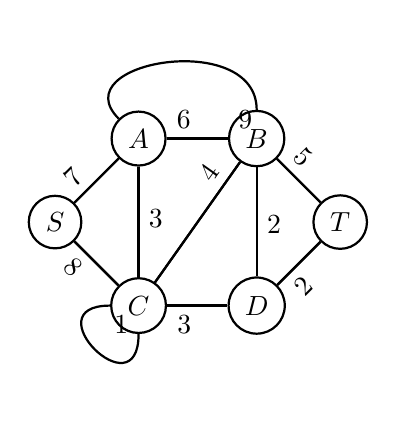
\begin{tikzpicture}[node distance={15mm}, thick, main/.style = {draw, circle}] 
\node[main] (1) {$S$}; 
\node[main] (2) [above right of=1] {$A$}; 
\node[main] (3) [below right of=1] {$C$}; 
\node[main] (4) [right of=2] {$B$}; 
\node[main] (5) [right of=3] {$D$}; 
\node[main] (6) [above right of=5] {$T$}; 
\draw (1) -- (2) ; 
\draw (1) -- (3); 
\draw (2) -- (3);
\draw (2) -- (4);
\draw (3) -- (4); 
\draw (3) -- (5); 
\draw (4) -- (5);
\draw (4) -- (6);
\draw (5) -- (6); 
\draw (3) to [out=180,in=270,looseness=5] (3); 
\draw (2) to [out=135,in=90,looseness=1.5] (4); 
\draw (1) -- node[midway, above right, sloped, pos=0] {7} (2); 
\draw (1) -- node[midway, below right, sloped, pos=0] {8} (3); 
\draw (2) -- node[midway, below right, pos=0.3] {3} (3); 
\draw (2) -- node[midway, above right, sloped, pos=0] {6} (4); 
\draw (3) -- node[midway, below right, sloped, pos=0] {3} (5); 
\draw (3) -- node[midway, above right, sloped, pos=0.7] {4} (4); 
\draw (4) -- node[midway, above right, pos=0.7] {2} (5); 
\draw (5) -- node[midway, below right, sloped, pos=0] {2} (6); 
\draw (4) -- node[midway, above right, sloped, pos=0] {5} (6); 
\draw (3) -- node[midway, below left, pos=0] {1} (3); 
\draw (2) -- node[midway,above right,sloped, pos=1] {9} (4); 
\end{tikzpicture} 

Step 1 - remove all loops and parallel edges.\\

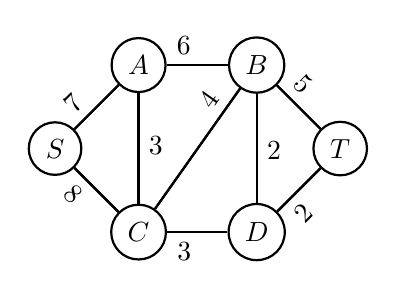
\begin{tikzpicture}[node distance={15mm}, thick, main/.style = {draw, circle}] 
\node[main] (1) {$S$}; 
\node[main] (2) [above right of=1] {$A$}; 
\node[main] (3) [below right of=1] {$C$}; 
\node[main] (4) [right of=2] {$B$}; 
\node[main] (5) [right of=3] {$D$}; 
\node[main] (6) [above right of=5] {$T$}; 
\draw (1) -- (2) ; 
\draw (1) -- (3); 
\draw (2) -- (3);
\draw (2) -- (4);
\draw (3) -- (4); 
\draw (3) -- (5); 
\draw (4) -- (5);
\draw (4) -- (6);
\draw (5) -- (6); 
\draw (1) -- node[midway, above right, sloped, pos=0] {7} (2); 
\draw (1) -- node[midway, below right, sloped, pos=0] {8} (3); 
\draw (2) -- node[midway, below right, pos=0.3] {3} (3); 
\draw (2) -- node[midway, above right, sloped, pos=0] {6} (4); 
\draw (3) -- node[midway, below right, sloped, pos=0] {3} (5); 
\draw (3) -- node[midway, above right, sloped, pos=0.7] {4} (4); 
\draw (4) -- node[midway, above right, pos=0.7] {2} (5); 
\draw (5) -- node[midway, below right, sloped, pos=0] {2} (6); 
\draw (4) -- node[midway, above right, sloped, pos=0] {5} (6); 
\end{tikzpicture} 

Step 2 - Arrange all edges in their increasing order of weights.\\
B-D=2, D-T=2, A-C=3, C-D=3, C-B=4, B-T=5, A-B=6, S-A=7, S-C=8\\

Step 3 - Add the edges which has least weights.\\
Start with B-D and D-T this has least weights which is 2.\\
\begin{tikzpicture}[node distance={15mm}, thick, main/.style = {draw, circle}] 
\node[main] (4) [right of=2] {$B$}; 
\node[main] (5) [right of=3] {$D$}; 
\node[main] (6) [above right of=5] {$T$}; 
\draw (4) -- (5);
\draw (5) -- (6); 
\draw (4) -- node[midway, above right, pos=0.7] {2} (5); 
\draw (5) -- node[midway, below right, sloped, pos=0] {2} (6); 
\end{tikzpicture} \\
Next cost is 3, the edges are A-C and C-D.\\
\begin{tikzpicture}[node distance={15mm}, thick, main/.style = {draw, circle}] 
\node[main] (2) [above right of=1] {$A$}; 
\node[main] (3) [below right of=1] {$C$}; 
\node[main] (4) [right of=2] {$B$}; 
\node[main] (5) [right of=3] {$D$}; 
\node[main] (6) [above right of=5] {$T$}; 
\draw (2) -- (3);
\draw (3) -- (5); 
\draw (4) -- (5);
\draw (5) -- (6); 
\draw (2) -- node[midway, below right, pos=0.3] {3} (3); 
\draw (3) -- node[midway, below right, sloped, pos=0] {3} (5); 
\draw (4) -- node[midway, above right, pos=0.7] {2} (5); 
\draw (5) -- node[midway, below right, sloped, pos=0] {2} (6); 
\end{tikzpicture} \\
Next cost is 4 which makes cycle so we discard the C-D edge. Ignore 5 and 6 also for the same reason.\\
Next cost is 7, 8 so the 7 is least smaller so we did not chose 8.\\
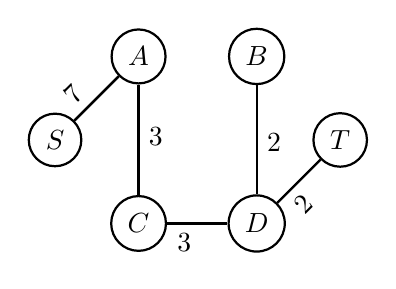
\begin{tikzpicture}[node distance={15mm}, thick, main/.style = {draw, circle}] 
\node[main] (1) {$S$}; 
\node[main] (2) [above right of=1] {$A$}; 
\node[main] (3) [below right of=1] {$C$}; 
\node[main] (4) [right of=2] {$B$}; 
\node[main] (5) [right of=3] {$D$}; 
\node[main] (6) [above right of=5] {$T$}; 
\draw (1) -- (2) ; 
\draw (2) -- (3);
\draw (3) -- (5); 
\draw (4) -- (5);
\draw (5) -- (6); 
\draw (1) -- node[midway, above right, sloped, pos=0] {7} (2); 
\draw (2) -- node[midway, below right, pos=0.3] {3} (3); 
\draw (3) -- node[midway, below right, sloped, pos=0] {3} (5); 
\draw (4) -- node[midway, above right, pos=0.7] {2} (5); 
\draw (5) -- node[midway, below right, sloped, pos=0] {2} (6); 
\end{tikzpicture} \\

Let's solve it using some simple definition:\\
e is the edge we reduce its weight\\
w(e) is the weight of the edge e\\
w(T) is the weight of tree T (sum of all edges)\\

I will prove it by contradiction Let's suppose that after decreasing the weight of of edge e from w(e) to w'(e) T is no more a minimal spanning tree, and T' is a minimal spanning tree.\\

First we consider the case where e belongs to T'.\\
$w(T')<w(T)$ by assumption w'(e) + w(T'-e) $<$ w'(e)+w(T-e)\\
w(T'-e) $<$ w(T-e) and that is true both in G and G, since {T'-e} and {T-e} are same in both graphs.\\
Then subsequently in G we have w(T'-e) $<$ w(T-e)\\
w(e) + w(T'-e) $<$ w(e) + w(T-e)\\
w(T') $<$ w(T) which means that G T is not a minimal spanning tree which is not correct.\\

Now we consider the case where e is not belongs to T'\\
Then in G' w(T') $<$ w(T) and by the same sequence w(T'-e) $<$ w(T-e) in both G and G' in G \\
we have consequently w(T'-e) + w(e) $<$ w(T-e) + w(e) and \\
if T'' === {T' + e} then w(T'') $<$ w(T) \\
which again contradicts the truth that T is MST in G.\\ 
 
Above is a graph with 6 vertices and 11 edges called G(V, E). And we have build a minimum spanning tree for G(V, E) called T(V', E') with a minimum of 6 vertices and 5 edges (6-1). \\

One More Simple Example\\
A Graph G:\\

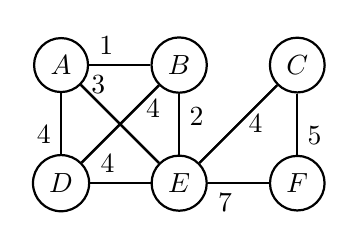
\begin{tikzpicture}[node distance={15mm}, thick, main/.style = {draw, circle}] 
\node[main] (1) {$A$}; 
\node[main] (2) [ right of=1] {$B$}; 
\node[main] (3) [ right of=2] {$C$}; 
\node[main] (4) [ below of=1] {$D$}; 
\node[main] (5) [right of=4]{$E$}; 
\node[main] (6) [right of=5]{$F$}; 
\draw (1) -- (2) ; 
\draw (1) -- (4);
\draw (1) -- (5); 
\draw (2) -- (4);
\draw (2) -- (5);
\draw (4) -- (5);
\draw (5) -- (3);
\draw (5) -- (6);
\draw (3) -- (6);
\draw (1) -- node[midway, above right, sloped, pos=0] {1} (2); 
\draw (2) -- node[midway, above right, pos=0.7] {2} (5); 
\draw (1) -- node[midway, above left, pos=1] {4} (4); 
\draw (1) -- node[midway, right, pos=0] {3} (5); 
\draw (4) -- node[midway, right, pos=0.7] {4} (2); 
\draw (4) -- node[midway, above right, pos=0] {4} (5);
\draw (5) -- node[midway, below right, sloped, pos=0] {7} (6);
\draw (5) -- node[midway, right, pos=0.5] {4} (3);
\draw (3) -- node[midway, above right, pos=1] {5} (6);
\end{tikzpicture} \\

Minimum spanning tree T:\\

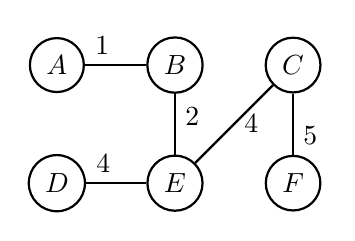
\begin{tikzpicture}[node distance={15mm}, thick, main/.style = {draw, circle}] 
\node[main] (1) {$A$}; 
\node[main] (2) [ right of=1] {$B$}; 
\node[main] (3) [ right of=2] {$C$}; 
\node[main] (4) [ below of=1] {$D$}; 
\node[main] (5) [right of=4]{$E$}; 
\node[main] (6) [right of=5]{$F$}; 
\draw (1) -- (2) ; 
\draw (2) -- (5);
\draw (4) -- (5);
\draw (5) -- (3);
\draw (3) -- (6);
\draw (1) -- node[midway, above right, sloped, pos=0] {1} (2); 
\draw (2) -- node[midway, above right, pos=0.7] {2} (5); 
\draw (4) -- node[midway, above right, pos=0] {4} (5);
\draw (5) -- node[midway, right, pos=0.5] {4} (3);
\draw (3) -- node[midway, above right, pos=1] {5} (6);
\end{tikzpicture} \\

Now take any vertex (x,y)[take (c,f) belongs to T and search for that vertex if (u,v) = (x,y) then reduce weight by k [ assume k = 1].\\
Now reduce weight of C,F by 1 will make it 4 . which also a MST.\\ 

If the edge weights are same, and you reduce weight of an edge which was already there in the MST, then since the total weight of the old MST has even reduced than it's previous value, therefore the MST will remain the same. But in case you reduce the edge weight of such an edge which was not there in the old MST, then the algorithm will be triggered to find the new MST, \\
following which the new MST will include the modified edge. if we remove any edge from the MST or decrease the weight of one edge of the tree.it is still a minimum spanning tree. 

\\Reference :- Krushkal's algorithm | Minimum Spanning Tree (MST) | Design & Algorithms | Lec-27 | Bhanu Priya, YouTube, March 22, 2018, https://www.youtube.com/watch?v=xn11tv6B4zw \\
Kruskal's Minimum Spanning Tree Algorithm: Greedy Algo-2, GeeksforGeeks, 
July 13, 2022, https://www.geeksforgeeks.org/kruskals-minimum-spanning-tree-algorithm-greedy-algo-2/ \\

  
\item (30 Pts.)  The single-source shortest path algorithm we studied
  requires time $O(|E|\log |V|+ |V|\log |V|)$ time to find the minimum
  distance $\delta(v_0, v_i)$ from the source $v_0$ to each node
  $v_i$. Checking the answer seems easier than finding it. Give an
  $O(|V|+|E|)$ time algorithm that, given a directed, connected,
  weighted graph (with nonnegative weights), and a sequence of
  distances $d_i$ for each $0\le i \le n$, will verify whether $d_i=
  \delta(v_0,v_i)$, i.e. whether $d_i$ really is the minimum distance
  from the source to vertex $v_i$. Argue the correctness of your
  algorithm (i.e. prove that (a) if the $d_i$'s are the shortest path
  values, your algorithm returns YES, and (b) if the di's are not
  correct shortest path values, your algorithm returns NO.) Explain
  why your algorithm is $O(|V|+|E|)$.
  
\item[Ans: ] We can calculate single-source shortest distances using the Bellman-Ford Algorithm in O(VE) time. We can perform better and use Dijkstra's technique to determine single-source shortest distances for a network without any negative weights in O(E + VlogV) time. We can calculate the single-source shortest distances for DAGs in O(V+E) time. Utilizing topological sorting is the plan. We set the distance to the source to 0 and the distances to all vertices to infinity. The graph is then sorted topologically, as we discover.\\
Once topological order (or a linear representation) has been established, each vertex is processed one at a time. We use the distance of the currently processed vertex to update the distances of every vertex that is adjacent to it.\\
Topological sorting for Directed Acyclic Graph (DAG) is a linear ordering of vertices such that for every directed edge u v, vertex u comes before v in the ordering. Topological Sorting for a graph is not possible if the graph is not a DAG.\\
Following is complete algorithm for finding shortest distances.\\ 
Initialize dist[] = {INF, INF, ….} and dist[s] = 0 where s is the source vertex.\\ 
Create a topological order of all vertices. \\
Do following for every vertex u in topological order. \\
Do following for every adjacent vertex v of u \\
if (dist[v] $>$ dist[u] + weight(u, v)) \\
dist[v] = dist[u] + weight(u, v) \\

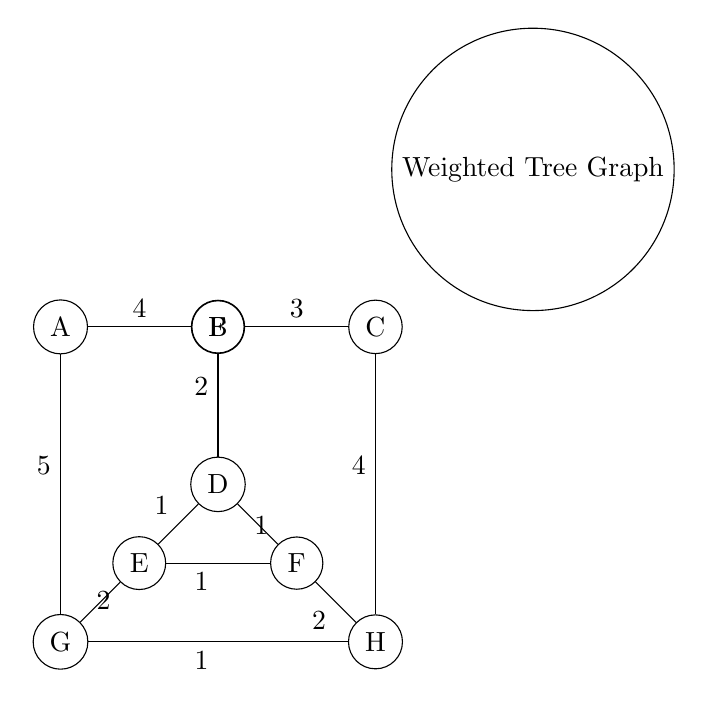
\begin{tikzpicture}
\draw 
(1, 1) node[circle, black, draw](g){G}
(1, 5) node[circle, black, draw](a){A}
(3, 3) node[circle, black, draw](d){D}
(3, 5) node[circle, black, draw](f){F}
(3, 5) node[circle, black, draw](b){B}
(5, 1) node[circle, black, draw](h){H}
(5, 5) node[circle, black, draw](c){C}
(2, 2) node[circle, black, draw](e){E}
(4, 2) node[circle, black, draw](f){F}

(7, 7) node[circle, black, draw](x){Weighted Tree Graph};

\draw[-] (a) -- node[above] {4} (b);
\draw[-] (b) -- node[above] {3} (c);
\draw (a) -- node[midway, above left, pos=0.5] {5} (g); 
\draw (b) -- node[midway, above left, pos=0.5] {2} (d); 
\draw (d) -- node[midway, above left, pos=0.5] {1} (e); 
\draw (d) -- node[midway, above left, pos=1] {1} (f); 
\draw (g) -- node[midway, below left, pos=0.5] {1} (h); 
\draw (c) -- node[midway, above left, pos=0.5] {4} (h); 
\draw (e) -- node[midway, below left, pos=0] {2} (g); 
\draw (f) -- node[midway, below left, pos=0.5] {2} (h); 
\draw (e) -- node[midway, below left, pos=0.5] {1} (f); 

\end{tikzpicture}

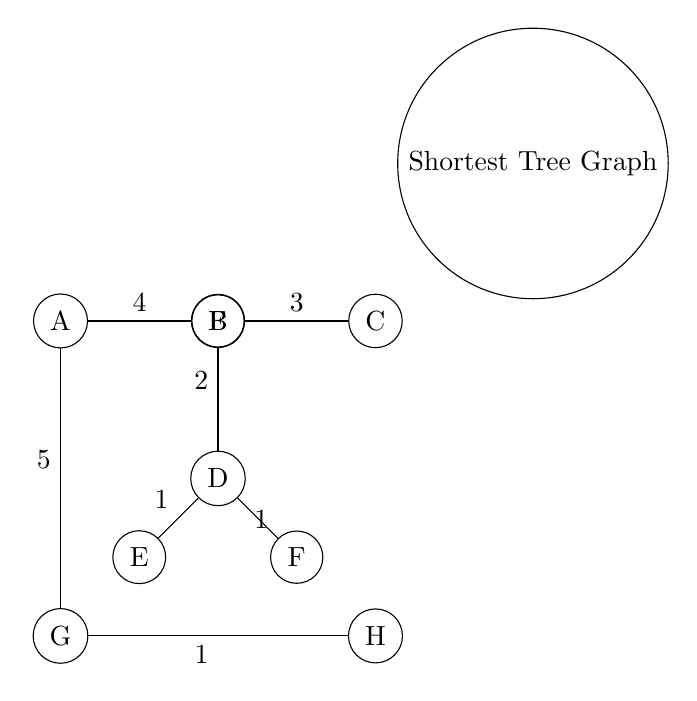
\begin{tikzpicture}
\draw 
(1, 1) node[circle, black, draw](g){G}
(1, 5) node[circle, black, draw](a){A}
(3, 3) node[circle, black, draw](d){D}
(3, 5) node[circle, black, draw](f){F}
(3, 5) node[circle, black, draw](b){B}
(5, 1) node[circle, black, draw](h){H}
(5, 5) node[circle, black, draw](c){C}
(2, 2) node[circle, black, draw](e){E}
(4, 2) node[circle, black, draw](f){F}

(7, 7) node[circle, black, draw](x){Shortest Tree Graph};

\draw[-] (a) -- node[above] {4} (b);
\draw[-] (b) -- node[above] {3} (c);
\draw (a) -- node[midway, above left, pos=0.5] {5} (g); 
\draw (b) -- node[midway, above left, pos=0.5] {2} (d); 
\draw (d) -- node[midway, above left, pos=0.5] {1} (e); 
\draw (d) -- node[midway, above left, pos=1] {1} (f); 
\draw (g) -- node[midway, below left, pos=0.5] {1} (h); 
\end{tikzpicture}

A shortest-paths tree rooted at vertex a for the graph from Figure weighted tree graph.\\
(a) Suppose it's known that di = $\delta(v0, vi).$ Then we simply can increase $\delta$ by one and find the distance. This gives a total running time of $O(|V |+1|E|)$, which is correct.\\
(b) Suppose it's not known whether di = $\delta$(v0, vi). Then there might be two possibilities.\\
(1) If vi is the next node in the minimum path from v0, then di must be less than $\delta$(v0, vi), and so di = $\delta$(v0, vi).\\
Alternatively (2) if vj is the next node in the actual minimum path from v0, then di must be greater than $\delta$(v0, vi), and so di $!= \delta$(v0, vi). Since we know that the first possibility is impossible (for if it had happened then it would have been confirmed by going to step 2 above), we can go to step 2 without further ado. This gives a total running time of $O(|V |+1|E|)$, which is correct.\\

The single source shortest path algorithm takes time $O(|E|log|V|+|V|log|V|)$ to find the minimum distance delta v0; vi) from source v0 to each node vi. \\
Using DFS depth first search with time complexity $O(|V| + |E|)$, we can determine the shortest routes. When the additional nodes are not available, DFS searches one path as far as it can before turning around. \\
We investigate untraveled side roads when going backward. DFS(V) Mark v as visited if it hasn't been before, then print (or otherwise process) v for each edge (V,W) In this approach, we can use DFS (W) to cover all the nodes with edges.\\

Given a directed graph where every edge has weight as either 1 or 2, find the shortest path from a given source vertex ‘s’ to a given destination vertex ‘t’. Expected time complexity is O(V+E).\\
Utilizing BFS is the plan. The path utilized in BFS always has the fewest edges between any two vertices, which is an important discovery about BFS. \\
Therefore, we can use BFS to determine the shortest path if all edges have the same weight. We may change the graph to solve this issue by dividing each edge with a weight of 2 into two edges with a weight of 1. We can use BFS to determine the shortest path in the changed graph.\\
For each source vertex, a new intermediate vertex must be added. It's easy to understand why. The graph gains new pathways from u to z and y to v that may not have existed in the original graph if we add an intermediate vertex x between u and v and if we add the same vertex between y and z.\\
Therefore, we require V more vertices in a graph containing V vertices. An example of the aforesaid concept in C++ is shown below. The technique shown below creates a graph with 2*V vertices and divides each edge (u, v) into two edges (u, u+V) and (u+V, w). So that a distinct intermediate vertex is added for every source vertex.\\

// Java program to find the shortest path from a given source vertex 's' to a given destination vertex 't'. Expected time complexity is O(V+E).\\
import java.util.*;\\
class GFG\\
{
	// This class represents a directed graph using adjacency\\
	// list representation\\
	static class Graph\\
	{
		int V; // No. of vertices\\
		Vector$<Integer>[]$ adj; // No. of vertices\\
		static int level;\\
		// Constructor\\
		@SuppressWarnings("unchecked")\\
		Graph(int V)\\
		{
			this.V = V;\\
			this.adj = new Vector[2 * V];\\
			for (int i = 0; i $<$ 2 * V; i++)\\
				this.adj[i] = new $Vector<>()$;\\
		}
		// adds an edge\\
		public void addEdge(int v, int w, int weight)\\
		{
			// split all edges of weight 2 into two edges of weight 1 each. \\
			The intermediate vertex number is maximum vertex number + 1, that is V.\\
			if (weight == 2)\\
			{
				adj[v].add(v + this.V);\\
				adj[v + this.V].add(w);\\
			} else // Weight is 1\\
				adj[v].add(w); // Add w to v's list.\\
		}
		// print shortest path from a source vertex 's' to destination vertex 'd'.\\
		public int printShortestPath(int[] parent, int s, int d)\\
		{
			level = 0;\\
			// If we reached root of shortest path tree\\
			if (parent[s] == -1)\\
			{
				System.out.printf("Shortest Path between"+"%d and %d is %s ", s, d, s);\\
				return level;\\
			}
			printShortestPath(parent, parent[s], d);\\
			level++;\\
			if (s $<$ this.V)\\
				System.out.printf("%d ", s);\\
			return level;\\
		}
		// finds shortest path from source vertex 's' to destination vertex 'd'.\\
		// This function mainly does BFS and prints the shortest path from src to dest. It is assumed that weight of every edge is 1\\		
		public int findShortestPath(int src, int dest)\\
		{
			boolean[] visited = new boolean[2 * this.V];\\
			int[] parent = new int[2 * this.V];\\
			// Initialize parent[] and visited[]\\
			for (int i = 0; i $<$ 2 * this.V; i++)\\
			{
				visited[i] = false;\\
				parent[i] = -1;\\
			}
			// Create a queue for BFS\\
			$Queue<Integer>$ queue = new $LinkedList<>()$;\\
			// Mark the current node as visited and enqueue it\\
			visited[src] = true;\\
			queue.add(src);\\
			while (!queue.isEmpty())\\
			{
				// Dequeue a vertex from queue and print it\\
				int s = queue.peek();\\
				if (s == dest)\\
					return printShortestPath(parent, s, dest);\\
				queue.poll();\\
				// Get all adjacent vertices of the dequeued vertex s\\
				// If a adjacent has not been visited, then mark it\\
				// visited and enqueue it\\
				for (int i : this.adj[s])\\
				{
					if (!visited[i])\\
					{
						visited[i] = true;\\
						queue.add(i);\\
						parent[i] = s;\\
					}
				}
			}
			return 0;\\
		}
	}

	// Driver Code\\
	public static void main(String[] args)\\
	{
		// Create a graph given in the above diagram\\
		int V = 4;\\
		Graph g = new Graph(V);\\
		g.addEdge(0, 1, 2);\\
		g.addEdge(0, 2, 2);\\
		g.addEdge(1, 2, 1);\\
		g.addEdge(1, 3, 1);\\
		g.addEdge(2, 0, 1);\\
		g.addEdge(2, 3, 2);\\
		g.addEdge(3, 3, 2);\\
		int src = 0, dest = 3;\\
		System.out.printf("\nShortest Distance between" + " %d and %d is %d\n", src, dest, g.findShortestPath(src, dest));\\
	}
}
\\

Output\\
Shortest Path between 0 and 3 is 0 1 3 \\
Shortest Distance between 0 and 3 is 3\\
The algorithm we've just described can be used to find the shortest path between any two nodes in a graph, weighted. In our example above, the distances are all positive integers, and so we can simply add them together. this approach is O(V+E) time complexity. In worst case, all edges are of weight 2 and we need to do O(E) operations to split all edges and 2V vertices, so the time complexity becomes O(E) + O(V+E) which is O(V+E).\\

BFS (Single Source Shortest Path in O(V+E))\\
for all v in vertices:\\
dist [v] = inf\\
dist[source] = 0;\\
deque d\\
d. push front (source)\\
while d.empty() == false:\\
vertex = get front element and pop as in BFS.\\
for all edges e of form (vertex , u):\\
if travelling e relaxes distance to u:\\
relax dist[u]\\
if e.weight = 1:\\
d.push back (u)\\
else:\\
d. push front (u)\\

\\Reference :- Figure 1. Graphs, Digraphs, and Networks - University of Washington, https://sites.math.washington.edu/~burke/crs/409/notes/graphs.pdf, August 20, 2022.\\
Shortest Path in a weighted Graph where weight of an edge is 1 or 2, GeeksforGeeks, June 30, 2022, https://www.geeksforgeeks.org/shortest-path-weighted-graph-weight-edge-1-2/\\
Single-Source Shortest Paths – Dijkstra's Algorithm, Techie Delight, November 06, 2021, https://www.techiedelight.com/single-source-shortest-paths-dijkstras-algorithm/\\
Shortest-Paths Trees - 國立臺灣大學, August 20,2022, https://www.csie.ntu.edu.tw/~kmchao/tree10spr/spt.pdf\\

\end{enumerate}
\end{document}
